\chapter{ZOZO}
\label{ch:zozosuit}

\section{Das Unternehmen ZOZO}
\label{sec:zozo}
ZOZO inc. ist ein japanisches Unternehmen, welches von Yusaku Maezawa im Jahr 1998 unter dem 
Namen \glqq{}Start today\grqq{} gegründet wurdet. Damals verkaufte das Unternehmen importierte 
CDs und Schallplatten. \newline
Das Unternehmen eröffnet im Jahr 2004 den Online-Shop ZOZOTOWN und stellt zwei Jahre später 
den verkauf importierter CDs komplett ein. \newline
Im Lauf der Jahre wurde der Online-Sohp immer weiter erweitert und weitere Unternehmen wurden in 
ZOZO inc. aufgenommen. \newline
Im Jahr 2018 veröffentlichte das Unternehmen den ZOZOSUIT. Ein Anzug und eine dazugehörige App, 
mit welcher der eigene Körper gemessen werden kann. Mithilfe dieser Daten konnten Nutzer 
maßgeschneiderte Kleidung im Online-Shop bestellen. \newline
Heute hat das Unternehmen 1297 Mitarbeiter und macht einen jährlichen Umsatz von 
1,1 Billionen Dollar \cite{misc:zozoforbes}.\cite{misc:zozohistory}

\pagebreak
\section{Der ZOZOSUIT}
\label{sec:zozosuit}

\begin{figure}[htpb]
    \centering
    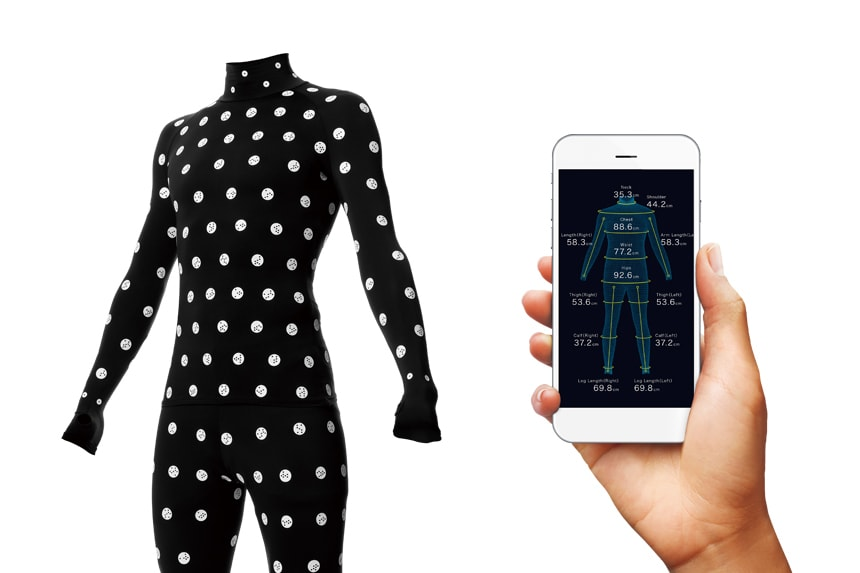
\includegraphics[width=0.7\textwidth]{zozosuit}
    \caption{Der ZOZOSUIT, Bildquelle: \cite{misc:zozopic}}
    \label{img:zozosuit}
\end{figure}
Der ZOZOSUIT ist ein enger Ganzkörperanzug mit gleichmäßig verteilten Punkten. Der Anzug wurde 
kostenlos an interessierte Menschen in der gesamten Welt versendet. \newline
Zu dem Suit gehört eine App, mit welcher Nutzer ein 360-Grad-Bild von sich selbst im ZOZOSUIT machen. 
Die App erkennt die auf dem ZOZOSUIT angebrachten Punkte und berechnet daraus die Maße 
des/der Trägers/-in.

Die berrechneten Maße können Nutzer hochladen und mit diesen Kleidung bei 
ZOZO inc. bestellen. Das Unternehmen versprach dabei, dass die bestellte Kleidung auf den Benutzer 
maßgeschneidert ist und innerhalb von zwei Wochen weltweit geliefert wird. \newline
In der Realität Betrug die Lieferzeit teils mehrere Monate. Zudem war die erhaltene Kleidung nicht passgenau. \newline
Dies sorgte für Enttäuschung und Unverständnis bei den Kunden, und als Resultat fiel der Wert von ZOZO-Aktien um circa 
50\% \cite{misc:zozoaktie}. \cite{misc:zozobad}

In Japan wurde die Benutzung des ZOZOSUIT bereits Ende 2018 abgeschafft und das Unternehmen entschuldigte sich für die große Enttäuschung.

Allerdings konnten die von Nutzern hochgeladenen Körperdaten weiterhin verwendet werden. Die Daten von millionen verschiedenster Körpertypen 
konnte ZOZO inc. dazu verwenden, die Produktion von nicht maßgeschneiderten Klamotten anzupassen. Somit wurde die Passgenauigkeit der von ZOZO 
produzierten Klamotten für den Durchschnitt der Bevölkerung erhöht.

\section{ZOZOSUIT 2}
\label{sec:zozosuit2}

\begin{figure}[H]
    \centering 
    \subfigure[Der ZOZOSUIT 2]{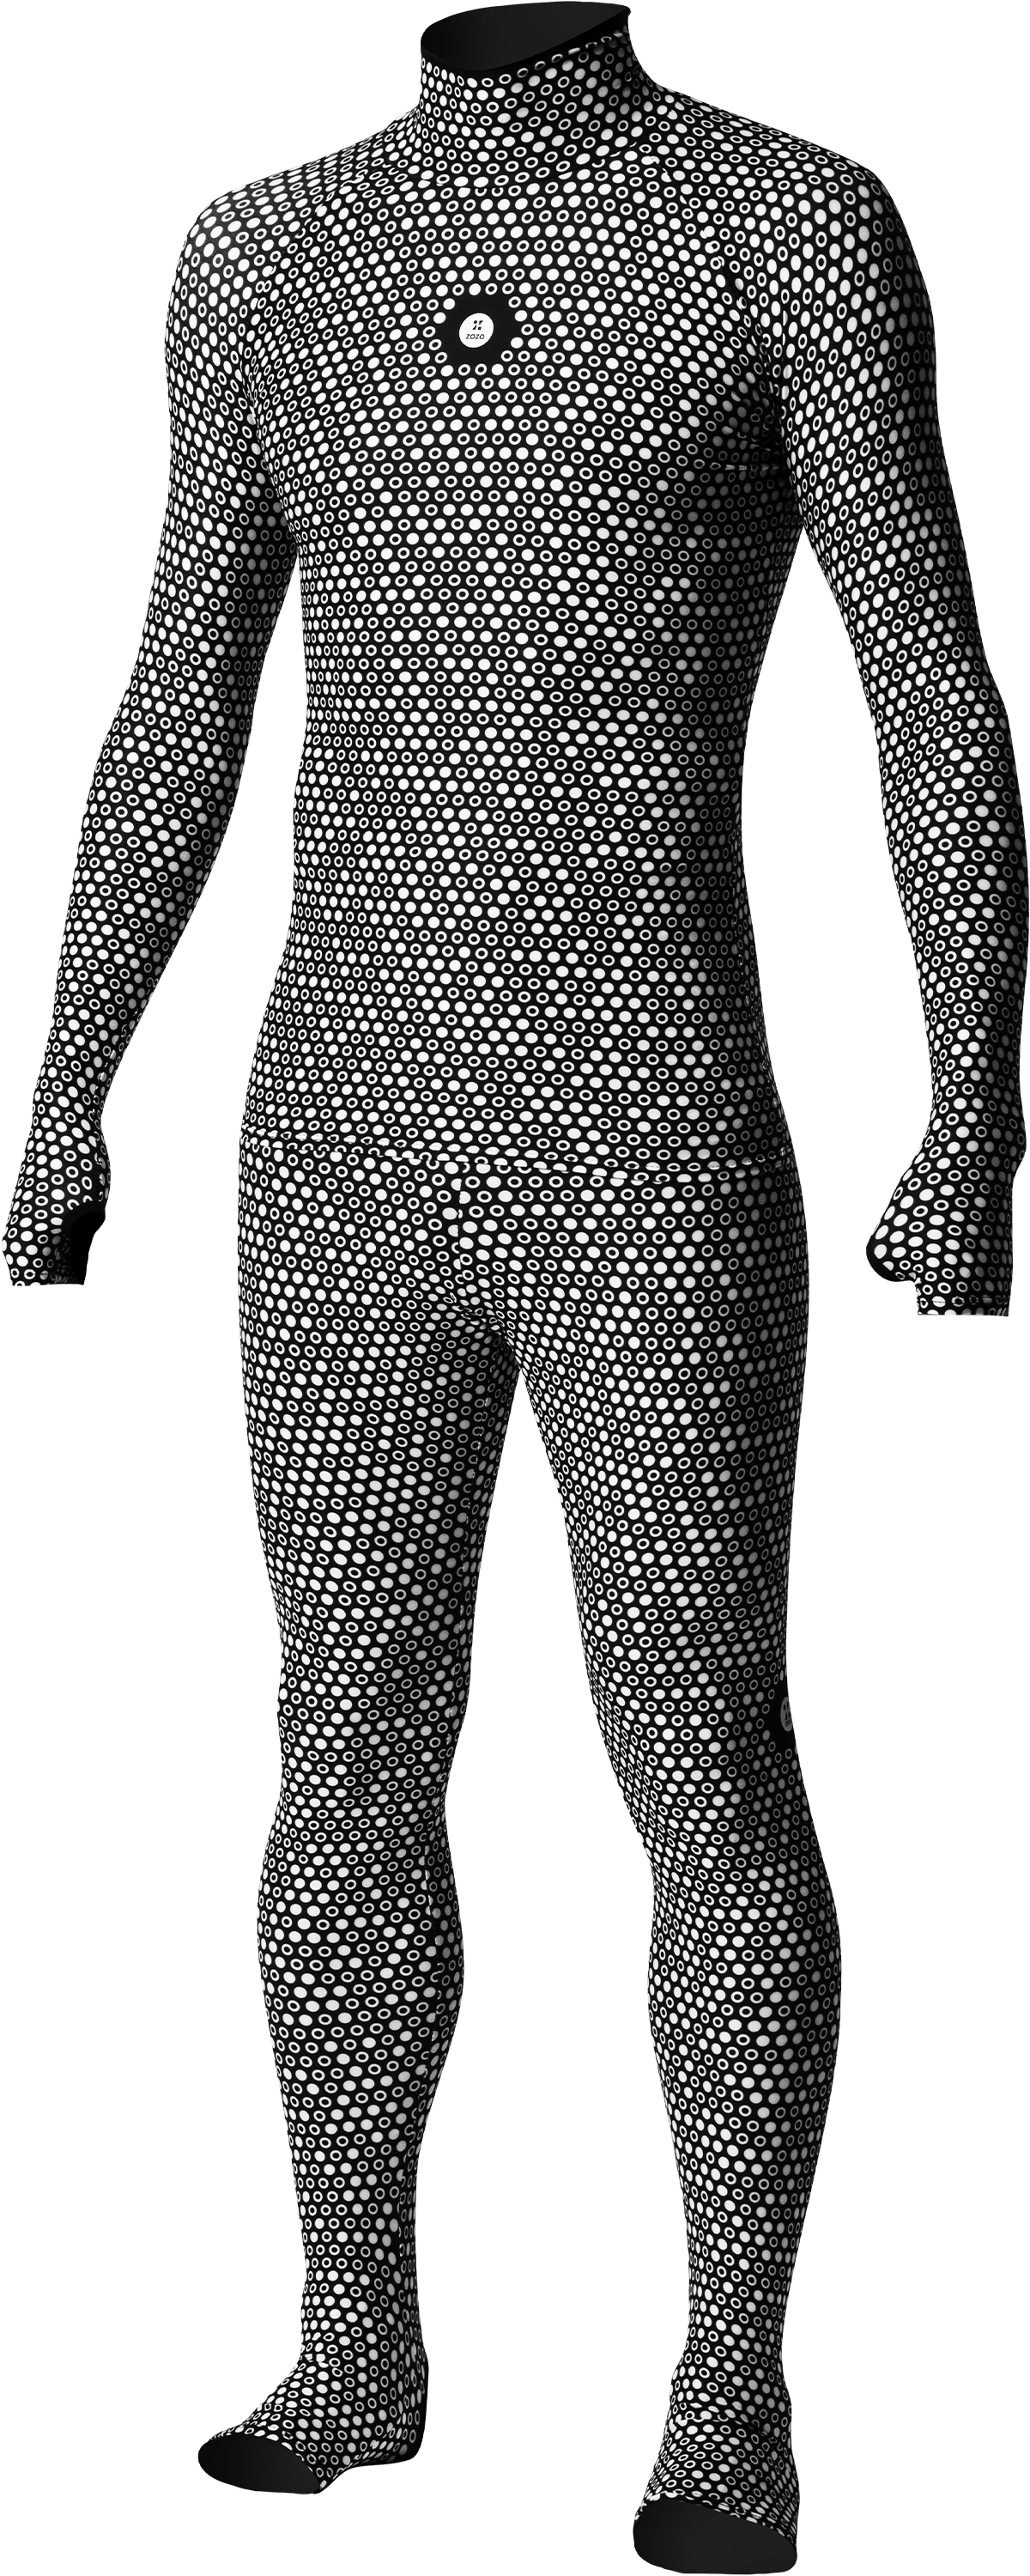
\includegraphics[width=0.3\textwidth]{zozosuit2_1}}\qquad
    \subfigure[Ausgewertete Punkte]{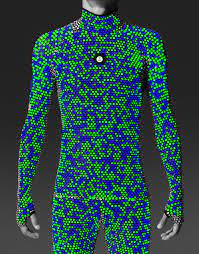
\includegraphics[width=0.45\textwidth]{zozosuit2_2}}
    \caption{Bildquelle: \cite{misc:zozopictwo}, \cite{misc:zozopictwopoints}} 
    \label{img:zozotwo}
  \end{figure}

Der ZOZOSUIT 2 verspricht das gleiche wie der ZOZOSUIT: ein hautenger Anzug mit gleichmäßigen Punkten 
und eine dazugehörige App, welche diese auswertet und anschließend ein 3D-Modell des Körpers anzeigt. \newline
Der ZOZOSUIT 2 besitzt im Vergleich zur ZOZOSUIT 50 mal mehr erkennbare Punkte. Zudem sind, laut Angaben von ZOZO inc. 
die zur Auswertung verwendeten Algorythmen verbessert worden. Zudem ist der Abstand der Punkte, welche zur Identifizierung 
der eigentlichen Messpunkte benötigt werden, von 0,2mm auf 0,4mm erhöht worden. Dies soll ermöglichen, dass Smartphones die 
Punkte besser erkennen. \cite{misc:zozotwo}

Wie sich im Verlauf dieser Studienarbeit herausstellt, würde die ZOZOSUIT 2 einige Probleme der Punkte-Erkennung und -Verarbeitung lösen (vgl. \ref{subsec:probleme}).